
\begin{figure}[H]
  {
    \setlength{\tabcolsep}{3.0pt}
    \setlength\cmidrulewidth{\heavyrulewidth} % Make cmidrule = 
    \begin{adjustbox}{width=3cm,center}
      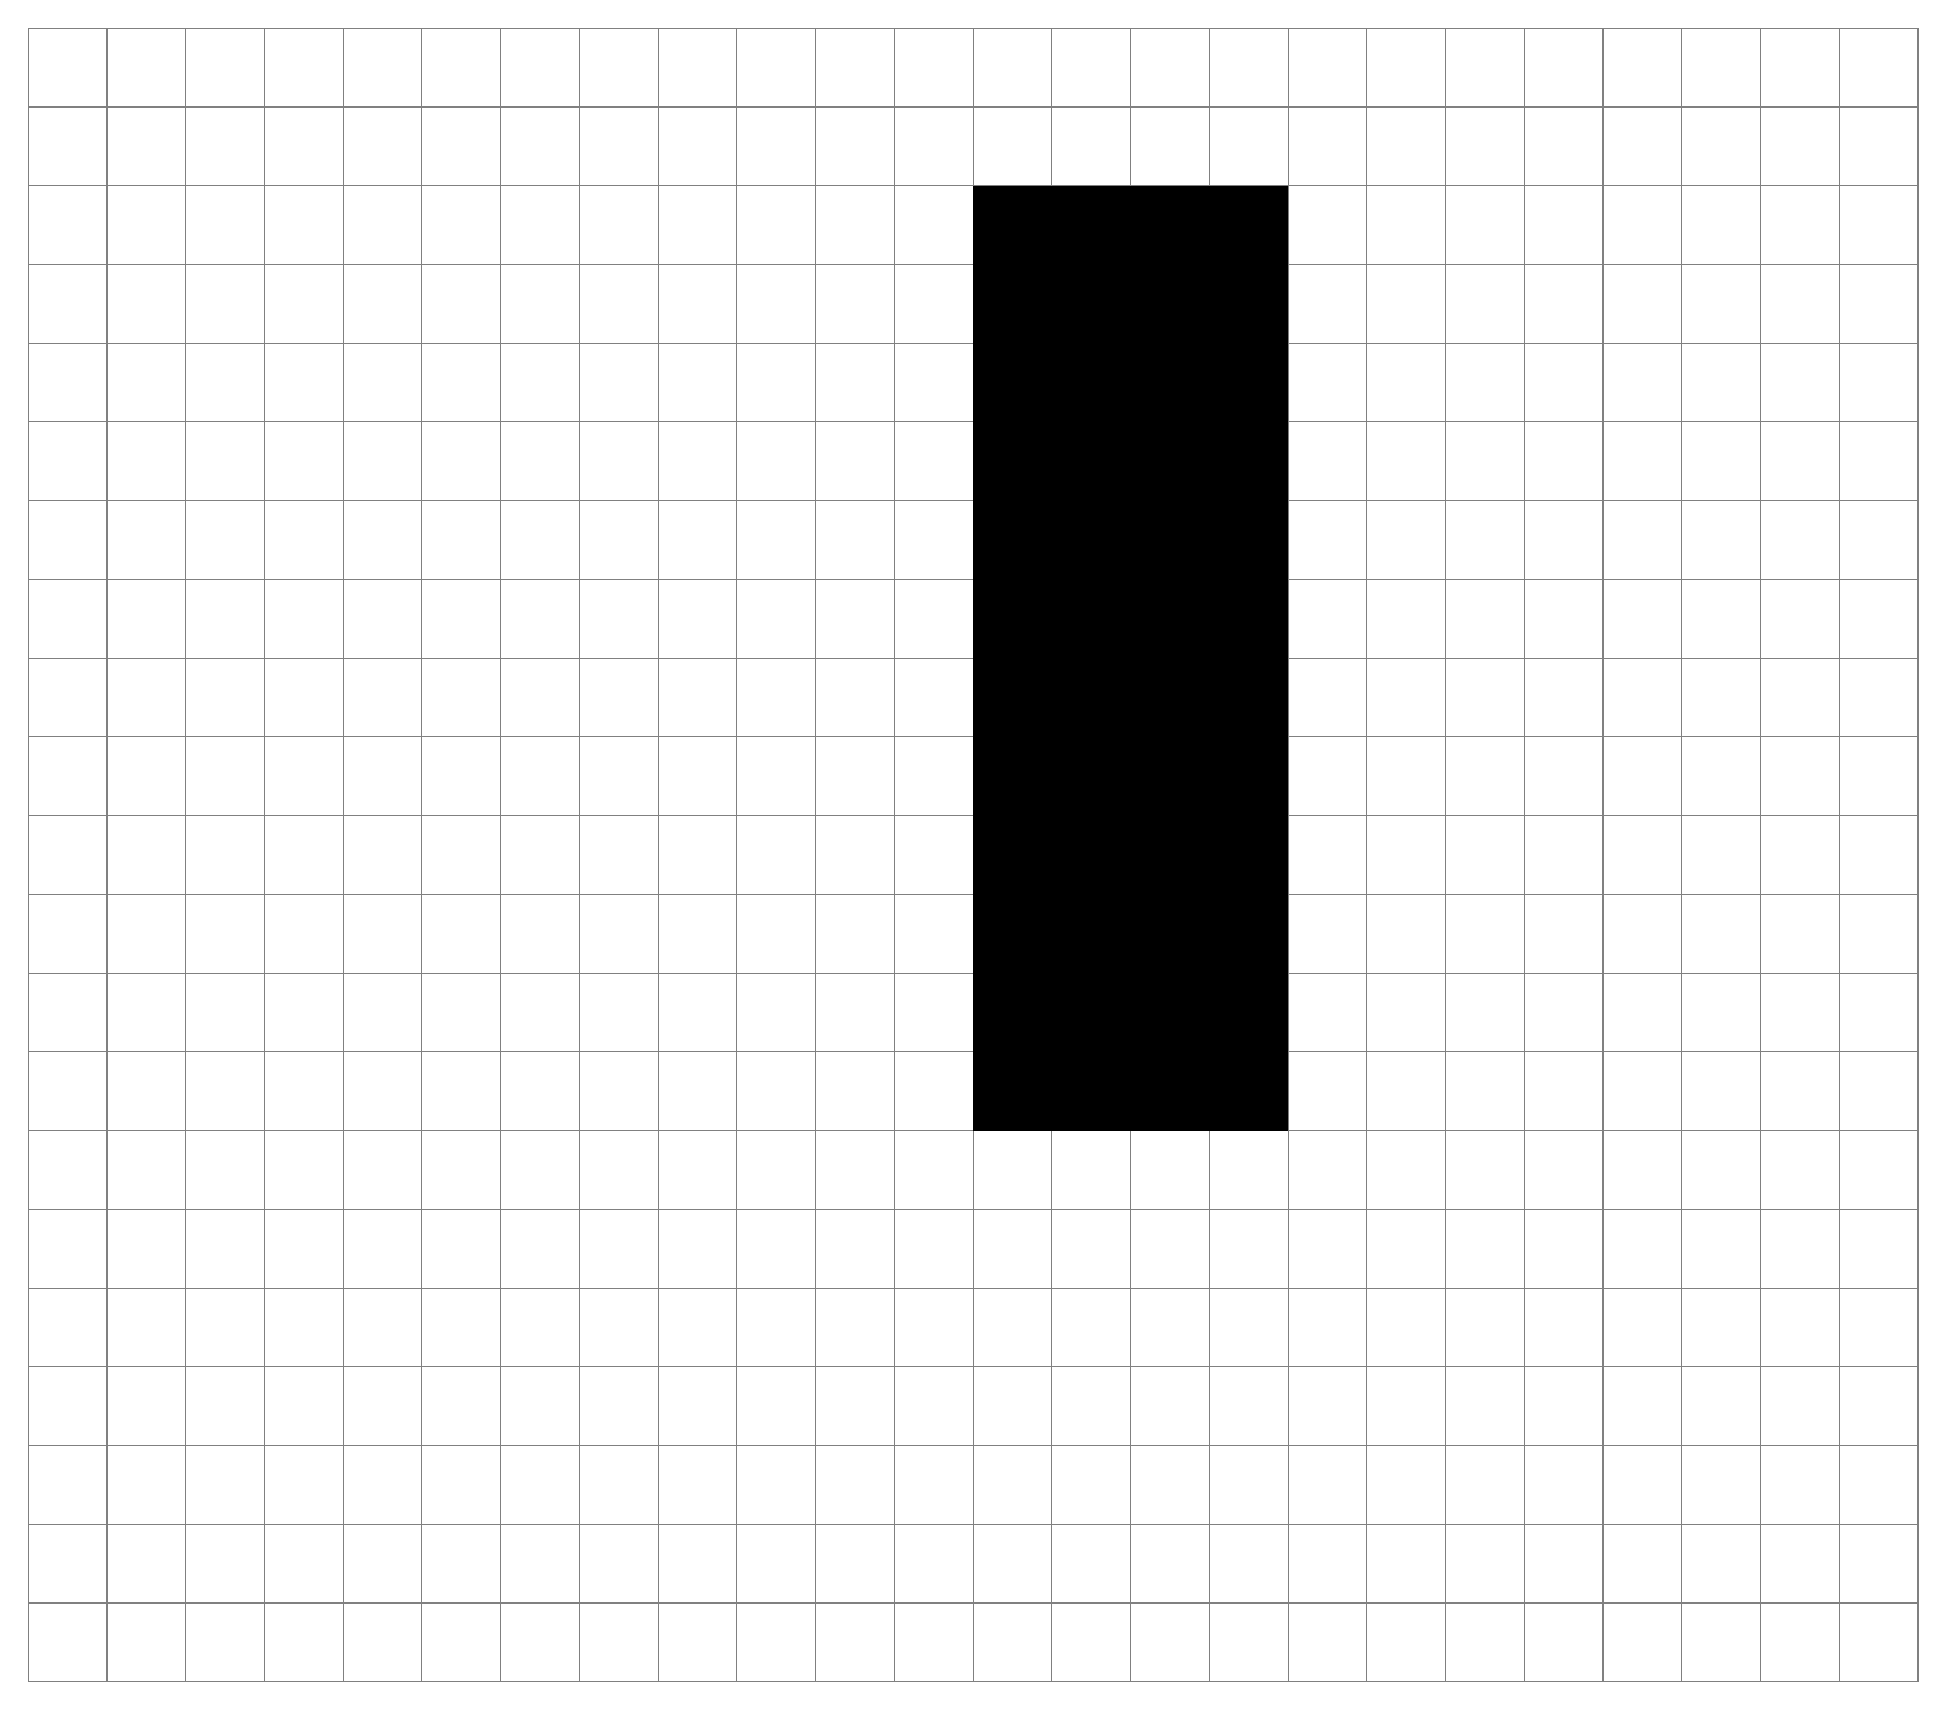
\begin{tikzpicture}

	\draw[step=1.0,gray,thin] (0,0) grid (24,21);
	\fill[\SPRITECOLOR] (12,18) rectangle ++ (1,1);
	\fill[\SPRITECOLOR] (13,18) rectangle ++ (1,1);
	\fill[\SPRITECOLOR] (14,18) rectangle ++ (1,1);
	\fill[\SPRITECOLOR] (15,18) rectangle ++ (1,1);
	\fill[\SPRITECOLOR] (12,17) rectangle ++ (1,1);
	\fill[\SPRITECOLOR] (13,17) rectangle ++ (1,1);
	\fill[\SPRITECOLOR] (14,17) rectangle ++ (1,1);
	\fill[\SPRITECOLOR] (15,17) rectangle ++ (1,1);
	\fill[\SPRITECOLOR] (12,16) rectangle ++ (1,1);
	\fill[\SPRITECOLOR] (13,16) rectangle ++ (1,1);
	\fill[\SPRITECOLOR] (14,16) rectangle ++ (1,1);
	\fill[\SPRITECOLOR] (15,16) rectangle ++ (1,1);
	\fill[\SPRITECOLOR] (12,15) rectangle ++ (1,1);
	\fill[\SPRITECOLOR] (13,15) rectangle ++ (1,1);
	\fill[\SPRITECOLOR] (14,15) rectangle ++ (1,1);
	\fill[\SPRITECOLOR] (15,15) rectangle ++ (1,1);
	\fill[\SPRITECOLOR] (12,14) rectangle ++ (1,1);
	\fill[\SPRITECOLOR] (13,14) rectangle ++ (1,1);
	\fill[\SPRITECOLOR] (14,14) rectangle ++ (1,1);
	\fill[\SPRITECOLOR] (15,14) rectangle ++ (1,1);
	\fill[\SPRITECOLOR] (12,13) rectangle ++ (1,1);
	\fill[\SPRITECOLOR] (13,13) rectangle ++ (1,1);
	\fill[\SPRITECOLOR] (14,13) rectangle ++ (1,1);
	\fill[\SPRITECOLOR] (15,13) rectangle ++ (1,1);
	\fill[\SPRITECOLOR] (12,12) rectangle ++ (1,1);
	\fill[\SPRITECOLOR] (13,12) rectangle ++ (1,1);
	\fill[\SPRITECOLOR] (14,12) rectangle ++ (1,1);
	\fill[\SPRITECOLOR] (15,12) rectangle ++ (1,1);
	\fill[\SPRITECOLOR] (12,11) rectangle ++ (1,1);
	\fill[\SPRITECOLOR] (13,11) rectangle ++ (1,1);
	\fill[\SPRITECOLOR] (14,11) rectangle ++ (1,1);
	\fill[\SPRITECOLOR] (15,11) rectangle ++ (1,1);
	\fill[\SPRITECOLOR] (12,10) rectangle ++ (1,1);
	\fill[\SPRITECOLOR] (13,10) rectangle ++ (1,1);
	\fill[\SPRITECOLOR] (14,10) rectangle ++ (1,1);
	\fill[\SPRITECOLOR] (15,10) rectangle ++ (1,1);
	\fill[\SPRITECOLOR] (12,9) rectangle ++ (1,1);
	\fill[\SPRITECOLOR] (13,9) rectangle ++ (1,1);
	\fill[\SPRITECOLOR] (14,9) rectangle ++ (1,1);
	\fill[\SPRITECOLOR] (15,9) rectangle ++ (1,1);
	\fill[\SPRITECOLOR] (12,8) rectangle ++ (1,1);
	\fill[\SPRITECOLOR] (13,8) rectangle ++ (1,1);
	\fill[\SPRITECOLOR] (14,8) rectangle ++ (1,1);
	\fill[\SPRITECOLOR] (15,8) rectangle ++ (1,1);
	\fill[\SPRITECOLOR] (12,7) rectangle ++ (1,1);
	\fill[\SPRITECOLOR] (13,7) rectangle ++ (1,1);
	\fill[\SPRITECOLOR] (14,7) rectangle ++ (1,1);
	\fill[\SPRITECOLOR] (15,7) rectangle ++ (1,1);

      \end{tikzpicture}
    \end{adjustbox}
  }\caption{SPINNING\_RING3}
\end{figure}
